\documentclass[reprint,amsmath,amssymb,aps,prb]{revtex4-2}

\usepackage{graphicx}
\usepackage{dcolumn}
\usepackage{bm}% bold math
\usepackage{braket}

\begin{document}

\title{Quantum Simulation of Black Hole Spacetime Using a One-Dimensional Lattice Fermion Model}

\author{Ann Author}
 \altaffiliation[Also at ]{Physics Department, XYZ University.}%Lines break automatically or can be forced with \\
\author{Second Author}%
 \email{Second.Author@institution.edu}
\affiliation{%
 Authors' institution and/or address
}%


\begin{abstract}
We study particle dynamics in a one-dimensional lattice Majorana-fermion model designed to emulate black hole and white-hole spacetimes. By encoding the effective metric into position-dependent lattice couplings, we analyze the low-momentum dispersion relation and the associated effective light-cone structure. Using real-space Bogoliubov--de Gennes diagonalization and wave packet time evolution, we show that packet trajectories agree with the corresponding geodesic motion for black hole profiles. We also extract the surface gravity from the near-horizon growth of the wave-packet standard deviation and compare the numerical result with the analytical scaling. For the white-hole geometry, we show that wave packet compression leads to finite-size reflection, with a stagnation time that scales logarithmically with the system size. We further clarify lattice-specific effects, including doubler-induced oscillations inside the black hole and partial transmission in the white-hole geometry for $p=1$. These results support lattice fermion models as practical platforms for quantum simulation of curved-spacetime particle dynamics while clarifying the lattice artifacts that control their range of validity.
\end{abstract}

\keywords{quantum simulation, analog gravity, lattice fermion model, black hole spacetime, Majorana fermion, wave packet dynamics, surface gravity, curved spacetime}
\maketitle

\section{INTRODUCTION}
Recent years have seen growing interest in quantum simulation as a powerful approach to investigating the dynamics of quantum many-body systems and quantum field theories that are difficult to treat using conventional numerical methods. In particular, significant progress has been made in reproducing complex physical phenomena with artificially engineered quantum systems. One notable direction is the simulation of physical processes in curved spacetime.

Quantum field theory in curved spacetime provides an important theoretical framework for understanding the interplay between gravity and quantum mechanics, including phenomena such as particle creation in the early universe and black hole evaporation~\cite{Wald2012,PhysRevLett.21.562}. A prominent example is Hawking radiation\cite{Hawking1975}, which is closely related to the black hole information paradox. However, direct experimental observation of quantum effects near black holes remains extremely challenging, leaving Hawking radiation without direct experimental verification.

To address this difficulty, increasing attention has been devoted to analog gravity, in which laboratory systems are used to mimic aspects of black hole spacetimes~\cite{Almeida2023}. Following Unruh's seminal proposal of an acoustic black hole~\cite{PhysRevLett.46.1351}, various platforms, including flowing fluids and Bose--Einstein condensates, have been explored to realize black hole-like phenomena in controllable experimental settings~\cite{Steinhauer2016}. These systems provide controlled settings for probing quantum field theory in effective curved spacetimes.

As an alternative approach, lattice-based methods encode spacetime geometry into spatially varying local couplings~\cite{PhysRevResearch.3.L022022,PhysRevLett.130.016701,marra2024metricinducednonhermitianphysics}. Such Hamiltonians are naturally suited to quantum-simulation platforms and allow different effective metrics to be implemented by changing coupling profiles~\cite{PhysRevLett.120.160403}. An early study in this direction is Ref.~\cite{PhysRevResearch.2.023107}, which investigated not only the Hawking temperature but also information-theoretic aspects of black holes by evaluating the entanglement entropy of the radiation and out-of-time-order correlators. The same work also discussed possible experimental implementations using optical lattices, superconducting qubits, and trapped ions. This proposal was later followed by an experimental realization on a superconducting processor~\cite{Shi2023}. Subsequent developments have further extended this line of research to quantum teleportation between black holes~\cite{PhysRevLett.130.016701,Daniel2025,daniel2025quantumteleportationsimulatedbinary} and simulations of $(2+1)$-dimensional black holes~\cite{benhemou2025probingquantumpropertiesblack}. These developments create opportunities for studying quantum dynamics in effective gravitational backgrounds within controllable lattice systems.

Within this context, a recent study proposed a method for simulating black hole spacetimes using a one-dimensional lattice fermion model~\cite{PhysRevResearch.7.023197}. This model can be extended to incorporate time-dependent spacetime backgrounds, enabling investigations of particle-production phenomena in curved spacetime. Such mechanisms are closely related to processes such as particle creation in the early universe and black hole evaporation and therefore offer a promising platform for exploring gravitational phenomena through quantum simulation. However, the extent to which the particle dynamics in this lattice model faithfully reproduce the physics of black hole spacetimes remains largely unexplored. Clarifying this point is essential for assessing the reliability of lattice-based approaches as platforms for simulating quantum-field dynamics in gravitational backgrounds.

In this work, we study particle dynamics in this one-dimensional lattice fermion model and clarify their correspondence with particle motion in an effective black-hole geometry.
To test this correspondence dynamically, we construct localized
quasiparticle wave packets in the lattice model and compare their
time evolution with geodesics of the target effective metric.
We further analyze how lattice-specific effects, such as fermion doubling and finite-size corrections, influence this correspondence.
Our results assess the regime in which the lattice fermion model reproduces black-hole analog dynamics and identify lattice effects relevant to quantum-simulation implementations.

This paper is organized as follows. In Sec. II, we introduce the one-dimensional lattice fermion model and explain how the effective metric and horizon structure emerge from its low-momentum dispersion. In Sec. III, we study wave packet dynamics in a black hole profile, compare the resulting trajectories with the corresponding geodesics, and analyze the role of fermion doubling. We also extract the surface gravity from wave packet broadening and then examine finite-size effects in a white-hole profile. Finally, Sec. IV summarizes our results and discusses future directions.

Throughout this paper, we use natural units with $\hbar=c=1$.

\section{LATTICE SIMULATOR OF
BLACK HOLES}
In this section, we introduce the one-dimensional lattice fermion model used to simulate black hole spacetime.
The basic idea is to encode the spacetime geometry into position-dependent hopping and pairing amplitudes.
We first summarize the correspondence between the continuum Majorana Hamiltonian in a curved background and the lattice Hamiltonian, and then discuss the locally defined dispersion relation that determines the effective light-cone structure.

We consider a massless Majorana field propagating on the effective spacetime described by the metric
\begin{align}
    ds^{2} =
    -\left[1-\beta^{2}(t,x)\right]dt^{2}
    - 2\beta(t,x)\,dt\,dx
    + dx^{2}.
    \label{simplified_metric}
\end{align}
On this background, the continuum Majorana Hamiltonian takes the form
\begin{align}
\begin{split}
H_{\rm cont}
= \int_{0}^{\ell} dx \Bigg[
&-\frac{1}{2}
\left(
\varphi^\dagger \partial_x \varphi^\dagger
-
\varphi \partial_x \varphi
\right) \\
&-\frac{i\beta(t,x)}{2}
\left(
\varphi^\dagger \partial_x \varphi
+
\varphi \partial_x \varphi^\dagger
\right)
\Bigg].
\end{split}
\label{continuum_hamiltonian_simplified}
\end{align}
Following the model introduced in Ref.~\cite{PhysRevResearch.7.023197}, the corresponding lattice model is described by the Hamiltonian
\begin{align}
\begin{split}
H
= - \frac{1}{2\varepsilon} \sum_{j=1}^{L} \Bigg[
& \frac12
\left(
c_{j-1}c_{j}
+
c_{j}c_{j+1}
\right)
\\
&+
\frac12
\left(
c_{j}^{\dagger}c_{j-1}^{\dagger}
+
c_{j+1}^{\dagger}c_{j}^{\dagger}
\right)
\\
&+
\frac{\beta(t,x_{j+\frac12})}{2}
\Big(
c_{j-1}^{\dagger}c_{j}
+
c_{j}^{\dagger}c_{j+1}
\\
&\hspace{3cm}
-
c_{j}^{\dagger}c_{j-1}
-
c_{j+1}^{\dagger}c_{j}
\Big)
\\
&+
\frac{p(t,x_{j+\frac{1}{2}})}{2}
\Big(
c_{j-1}^{\dagger}c_{j}
+
c_{j}^{\dagger}c_{j+1}
\\
&\hspace{3cm}
+
c_{j}^{\dagger}c_{j-1}
+
c_{j+1}^{\dagger}c_{j}
\Big)
\\
&+
p(t,x_{j+\frac{1}{2}})
\left(
1-2c_{j}^{\dagger}c_{j}
\right)
\Bigg].
\end{split}
\label{symmetrized_lattice_hamiltonian}
\end{align}
Here, $\varepsilon$ denotes the lattice spacing, $x_j=\varepsilon j$, and the continuum system size is $\ell=\varepsilon L$.
The continuum field $\varphi$ and the lattice fermion operator $c_j$ are related by $c_j=\sqrt{\varepsilon}\,\varphi(x_j)$.
They obey the canonical anticommutation relations
$\{\varphi(t,x),\varphi^{\dagger}(t,y)\}=\delta(x-y)$ and
$\{c_j,c_l^{\dagger}\}=\delta_{jl}$, with all other anticommutators vanishing.
The function $p(t,x_j)$ represents a freedom in the lattice realization.
Although different choices of $p$ define distinct finite-size lattice Hamiltonians, they converge to the same continuum field theory in the limit $L\to\infty$ with fixed $\ell$.

In the following, we provide an intuitive explanation of how the lattice model introduced above simulates black hole spacetime.
We first impose periodic boundary conditions and diagonalize the Hamiltonian in momentum space to obtain the dispersion relation.
For site-dependent couplings a global Fourier transform is not available.
We therefore use a local-homogeneity approximation, treating $\beta$ as constant over a sufficiently small spatial region.

Under this local-homogeneity assumption, each region in which $\beta$ can be regarded as constant is assumed to contain a sufficiently large number of sites.
Denoting this number by $L'$, we introduce the Fourier transformation
\begin{align}
c_j
&=
\frac{1}{\sqrt{L'}}
\sum_{k\in\mathcal{K}}
e^{ikj}c_k,
\notag\\
\mathcal{K}
&=
\left\{
\frac{2\pi}{L'}n
\,\bigg|\,
n=-\frac{L'}{2}+1,\ldots,\frac{L'}{2}
\right\}.
\label{eq:fourier_local}
\end{align}
Here, $L'$ is taken to be sufficiently large so that boundary effects can be neglected.
The Hamiltonian can then be decomposed into independent momentum sectors as
\begin{align}
H
=
\sum_{k\in\mathcal{K}}
\vec{c}_k^{\,\dagger}
\mathcal{H}(k)
\vec{c}_k,
\qquad
\vec{c}_k
\equiv
\begin{pmatrix}
c_k\\
c_{-k}^{\dagger}
\end{pmatrix}.
\end{align}

Fig.~\ref{fig:dispersion}(a) shows the dispersion relations at representative values of $\beta$ for both $p=1$ (top row) and $p=0$ (bottom row), with the associated spatial positions indicated in Fig.~\ref{fig:dispersion}(b).
Since $v_g=\partial E/\partial k$, the slopes near $k=0$ reproduce the effective light-cone structure expected in the continuum limit, as shown in Fig.~\ref{fig:dispersion}(c), and this low-momentum behavior is common to both choices of $p$.
On the other hand, the $p=0$ lattice Hamiltonian always has a doubler branch near $k=\pi$.
For $p=1$, the doubler branch is absent in the asymptotically flat low-energy spectrum but appears inside the horizon, where $|\beta|>1$.
Thus, wave packet dynamics can involve lattice-artifact doubler modes for both choices of $p$.

\begin{figure}[t]
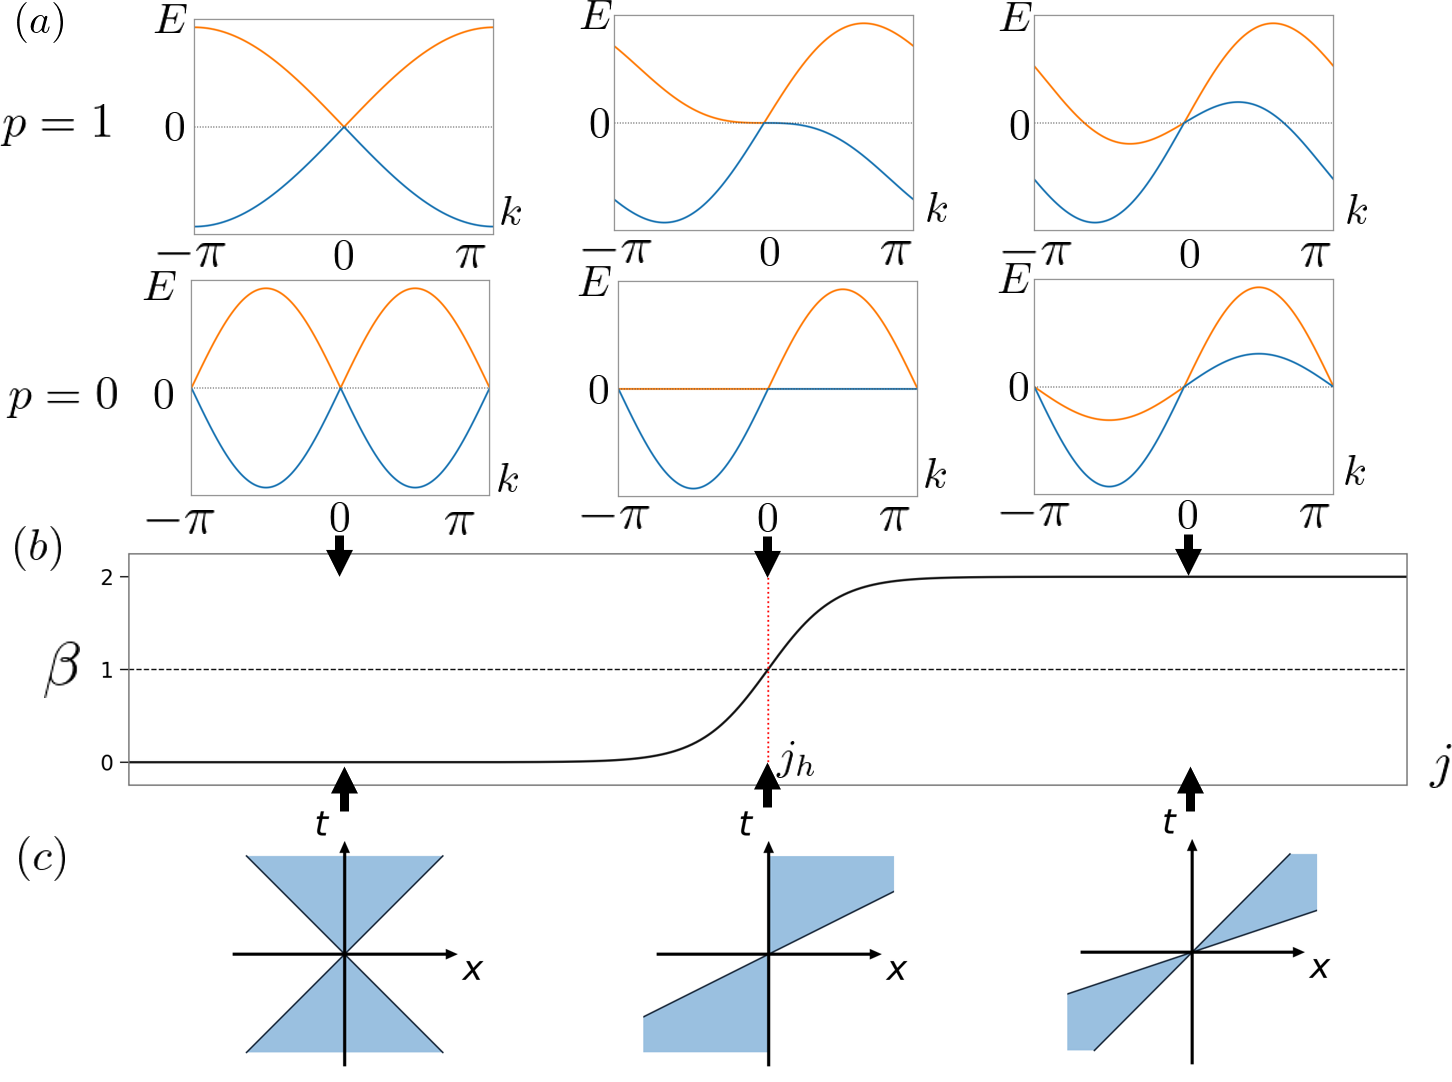
\includegraphics[width=\linewidth]{figure/dispersion.png}
\caption{Connection between the local dispersion relation of the lattice Hamiltonian and the effective light-cone structure. (a) Dispersion relations at representative values of $\beta$: top row for $p=1$ and bottom row for $p=0$. The slopes near $k=0$ give the low-momentum group velocities and reproduce the same effective light-cone structure for both choices of $p$. For $p=0$, an additional low-energy branch appears near $k=\pi$, indicating a fermion doubler; for $p=1$, this doubler branch is absent in the asymptotically flat low-energy spectrum but emerges inside the horizon, where $|\beta|>1$. (b) Spatial profile of $\beta(j)$. The arrows indicate the spatial positions used in the dispersion plots in (a), and the dashed line marks $\beta=-1$ for the displayed profile. (c) Effective light cones determined by the low-momentum group velocities. In the region $\beta<-1$, both characteristic velocities are negative.}
\label{fig:dispersion}
\end{figure}

In the preceding discussion, we obtained an approximate description of the particle dynamics by assuming that $\beta$ is locally constant.
We now consider the full black hole spacetime by retaining the site dependence of the coupling constants and diagonalizing the Hamiltonian in real space.

The quadratic Hamiltonian can be expressed in BdG form as
\begin{equation}
H = \frac{1}{2}\,\Psi^{\dagger}\,\mathcal{H}_{\mathrm{BdG}}\,\Psi + \mathrm{const},
\end{equation}
where
\begin{equation*}
\Psi = \bigl(c_{1},\,\ldots,\,c_{L},\,c_{1}^{\dagger},\,\ldots,\,c_{L}^{\dagger}\bigr)^{\mathsf T}.
\end{equation*}
We diagonalize the BdG Hamiltonian with a unitary matrix $U$ defined by $\Psi=U\Gamma$, where
\begin{align}
    \Gamma =
    \left(
    \gamma_1,\ldots,\gamma_L,
    \gamma_1^\dagger,\ldots,\gamma_L^\dagger
    \right)^T .
\end{align}
The Hamiltonian is then written as
\begin{align}
    H = \sum_{n=1}^{L} E_n \gamma_n^\dagger \gamma_n + \mathrm{const}.
\end{align}
Since the occupation numbers $\gamma_n^\dagger\gamma_n$ are conserved, the time evolution can be studied within the single-particle sector spanned by
\begin{align}
\ket{\boldsymbol{\gamma_n}}
=
\gamma_n^\dagger \ket{0},
\qquad
n=1,\ldots,L.
\end{align}

To compare lattice wave packet dynamics with geodesic motion, it is useful to prepare wave packets with a definite propagation direction. The original fermion operator $c_j$ does not directly separate the right- and left-moving components. We therefore introduce the Majorana-like mode operators
\begin{equation}
\chi_j^\pm =
\frac{1}{\sqrt{2}}
\left(
e^{\pm i\pi/4} c_j
+
e^{\mp i\pi/4} c_j^\dagger
\right).
\label{eq:chi_pm_def}
\end{equation}
These operators satisfy $\{\chi_i^\pm,\chi_j^\pm\}=\delta_{ij}$ and $\{\chi_i^+,\chi_j^-\}=0$, and therefore provide a convenient real-fermion basis for separating the right- and left-moving components of the lattice Hamiltonian.

In terms of these operators, the local Hamiltonian density can be separated as
\begin{equation}
\mathcal{H}_j = \mathcal{H}_j^+ + \mathcal{H}_j^- + \mathcal{H}_j^\pm ,
\label{eq:H_decomposition}
\end{equation}
where $\mathcal{H}_j^+$ and $\mathcal{H}_j^-$ denote the single-component terms for $\chi^+$ and $\chi^-$, respectively, while $\mathcal{H}_j^\pm$ describes the coupling between them. Explicitly, these terms are given by
\begin{align}
\mathcal{H}_j^+
&=
-\frac{i}{4\varepsilon}
(1+\beta_{j+\frac{1}{2}})
\left(
\chi_{j-1}^+\chi_j^+
+
\chi_j^+\chi_{j+1}^+
\right),
\label{eq:H_plus}
\\
\mathcal{H}_j^-
&=
\frac{i}{4\varepsilon}
(-1+\beta_{j+\frac{1}{2}})
\left(
\chi_{j-1}^-\chi_j^-
+
\chi_j^-\chi_{j+1}^-
\right),
\label{eq:H_minus}
\\
\mathcal{H}_j^\pm
&=
-\frac{i p}{4\varepsilon}
\left[
\chi_{j-1}^+\chi_j^-
+
\chi_{j-1}^-\chi_j^+
+
\chi_j^+\chi_{j+1}^-
+
\chi_j^-\chi_{j+1}^+
\right]
\nonumber\\
&\quad
-
\frac{p-\varepsilon m}{\varepsilon}
\chi_j^+\chi_j^-.
\label{eq:H_pm}
\end{align}
Here $\beta_{j+\frac{1}{2}}\equiv\beta(t,x_{j+\frac{1}{2}})$.
Thus, when $p=0$ and $m=0$, the $\chi^+$ and $\chi^-$ components are decoupled.

The interpretation of these two components becomes clear from the Heisenberg equation of motion.
After summing over site-centered densities, the bond coefficient contains the averaged factor
\begin{equation}
    \bar{\beta}_{j+\frac{1}{2}}
    :=
    \frac{\beta_{j+\frac{1}{2}}+\beta_{j+\frac{3}{2}}}{2}.
\end{equation}
Using the lattice Hamiltonian, one obtains
\begin{align}
i\frac{\partial}{\partial t}\chi_j^+
&=
[\chi_j^+,H]
\nonumber\\
&=
-\frac{i}{2\varepsilon}
\left[
(1+\bar{\beta}_{j+\frac{1}{2}})\chi_{j+1}^+
-
(1+\bar{\beta}_{j-\frac{1}{2}})\chi_{j-1}^+
\right]
\nonumber\\
&\quad
-
\frac{i p}{2\varepsilon}
\left(
\chi_{j+1}^-
-
\chi_{j-1}^-
\right)
-
\frac{p-\varepsilon m}{\varepsilon}\chi_j^-,
\nonumber\\
i\frac{\partial}{\partial t}\chi_j^-
&=
[\chi_j^-,H]
\nonumber\\
&=
\frac{i}{2\varepsilon}
\left[
(-1+\bar{\beta}_{j+\frac{1}{2}})\chi_{j+1}^-
-
(-1+\bar{\beta}_{j-\frac{1}{2}})\chi_{j-1}^-
\right]
\nonumber\\
&\quad
-
\frac{i p}{2\varepsilon}
\left(
\chi_{j+1}^+
-
\chi_{j-1}^+
\right)
+
\frac{p-\varepsilon m}{\varepsilon}\chi_j^+ .
\label{eq:chi_eom_lattice}
\end{align}
In the massless and decoupled limit, $m=p=0$, these equations reduce to transport equations for each component.

In the wave packet simulations below, the initial state is constructed by applying a Gaussian superposition of either $\chi_j^+$ or $\chi_j^-$ to the BdG vacuum,
\begin{equation}
|\psi(0)\rangle
=
\sum_j G(j)\chi_j^\pm |\mathrm{vac}\rangle .
\label{eq:initial_state_chi}
\end{equation}
where the Gaussian envelope $G(j)$ is defined as
\begin{align}
G(j) = \mathcal{N}
\exp\!\left[-\frac{(j - j_{0})^{2}}{2\sigma^{2}}\right],
\qquad
\sum_{j}|G(j)|^2=1.
\label{eq:gaussian}
\end{align}
Here, $j_{0}$ and $\sigma$ denote the center position and standard deviation of the wave packet, respectively, and $\mathcal{N}$ is the normalization constant. This construction selectively excites either the right-moving or left-moving mode while keeping the momentum distribution concentrated near the low-momentum region, where the lattice dispersion reproduces the continuum curved-spacetime dynamics. The subsequent time evolution of these wave packets is then compared with the corresponding geodesic motion.
We monitor the wave packet dynamics through the vacuum-subtracted local energy densities.


\section{DYNAMICS OF PARTICLES IN BLACK- AND WHITE-HOLE GEOMETRIES}
\label{sec:dynamics}
Using the discrete model, we analyze the dynamics of a wave packet. Numerical simulations reveal that the wave packet follows the corresponding geodesic trajectory. In addition, we demonstrate that the surface gravity of the black hole can be extracted from the simulation results.

Throughout the following analysis, we take the function $\beta$, which determines the metric, to be
\begin{align}
\beta(x) = A\tanh\left[B(x-x_0)\right] + C,
\end{align}
where $x_0$ is the inflection point of the $\tanh$ profile, and $A$, $B$, and $C$ are real constants.
As follows from the equations of motion for $\chi_j^\pm$ in Eq.~\eqref{eq:chi_eom_lattice}, the horizon condition is set by the vanishing of the characteristic velocity of the wave packet component under consideration, with $\beta=-1$ for the $\chi^+$ component and $\beta=1$ for the $\chi^-$ component.
Whether the resulting horizon is black-hole-like or white-hole-like depends on both the propagating component and the sign of $\partial_x\beta$ at the horizon.
We denote the horizon position by $x_h$, with $j_h=Lx_h/\ell$.
Note that $x_0$ coincides with a horizon only when $|C|=1$.

Unless otherwise noted, we set $L=300$, $m=0$, and impose open boundary conditions.

\subsection{Black Hole}
For the black hole wave packet dynamics shown in Figs.~\ref{fig:bh_p0} and \ref{fig:bh_p1}, we use $A=0.6$, $B=3$, $C=0.6$, and $\ell=2\pi$. In panels (a,b), we set $x_0=2\ell/3$, for which the event horizon where $\beta=1$ lies at $j_h\approx213$; in panels (c,d), we set $x_0=\ell/3$, for which the event horizon lies at $j_h\approx113$. The wave packets in Figs.~\ref{fig:bh_p0}(a,b) and \ref{fig:bh_p1}(a,b) are initially placed outside the black hole, whereas those in Figs.~\ref{fig:bh_p0}(c,d) and \ref{fig:bh_p1}(c,d) are initially placed inside the black hole.

\begin{figure*}[t]
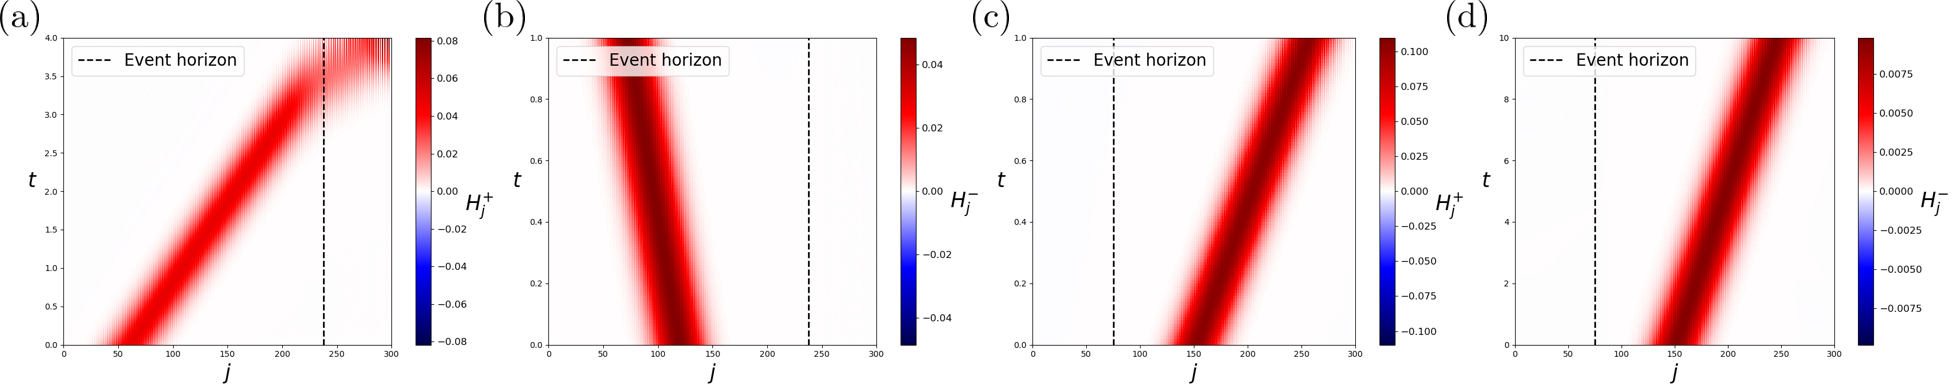
\includegraphics[width=\linewidth]{figure/p=0_BH.png}
\caption{Wave packet dynamics for the black hole profile with $p=0$. The system parameters are $L=300$, $\ell=2\pi$, and $\beta(x)=A\tanh[B(x-x_0)]+C$ with $A=0.6$, $B=3$, and $C=0.6$. In (a,b), $x_0=2\ell/3$ and the event horizon is at $j_h\approx213$; in (c,d), $x_0=\ell/3$ and the event horizon is at $j_h\approx113$. (a) Packet initialized outside the horizon with ingoing group velocity ($j_0=30$, $\sigma=0.05L$). (b) Packet initialized outside the horizon with outgoing group velocity ($j_0=40$, $\sigma=0.05L$). (c) Packet initialized inside the horizon with a right-moving initial spinor ($j_0=180$, $\sigma=0.05L$). (d) Packet initialized inside the horizon with a left-moving initial spinor ($j_0=180$, $\sigma=0.05L$). Red dashed lines indicate the event horizon, and cyan curves indicate the corresponding null geodesics $dx/dt=\beta(x)\pm1$.}
\label{fig:bh_p0}
\end{figure*}
We first examine the motion of the wave packet for the case $p=0$.
Fig.~\ref{fig:bh_p0} shows the time evolution of wave packets for several initial conditions.
The event horizon is indicated by the red line, while the geodesic is shown by the light-blue curve.
The region to the right of the event horizon corresponds to the black hole interior.
Figs.~\ref{fig:bh_p0}(a,b) show that wave packets initially placed outside the black hole follow the corresponding geodesic trajectories for both ingoing and outgoing motion.
Figs.~\ref{fig:bh_p0}(c,d) show the time evolution of a wave packet initially placed inside the black hole.
Inside the event horizon, both characteristic velocities are positive in this setup, so wave packets propagate only toward increasing $x$.
Thus, the wave packet is expected to propagate only to the right.
The numerical results show that both the right-moving mode in Fig.~\ref{fig:bh_p0}(c) and the left-moving mode in Fig.~\ref{fig:bh_p0}(d) propagate in the rightward direction.
The initial state was chosen with $j_0=180$, and the standard deviation was set to $\sigma=0.05L$.

\begin{figure*}[t]
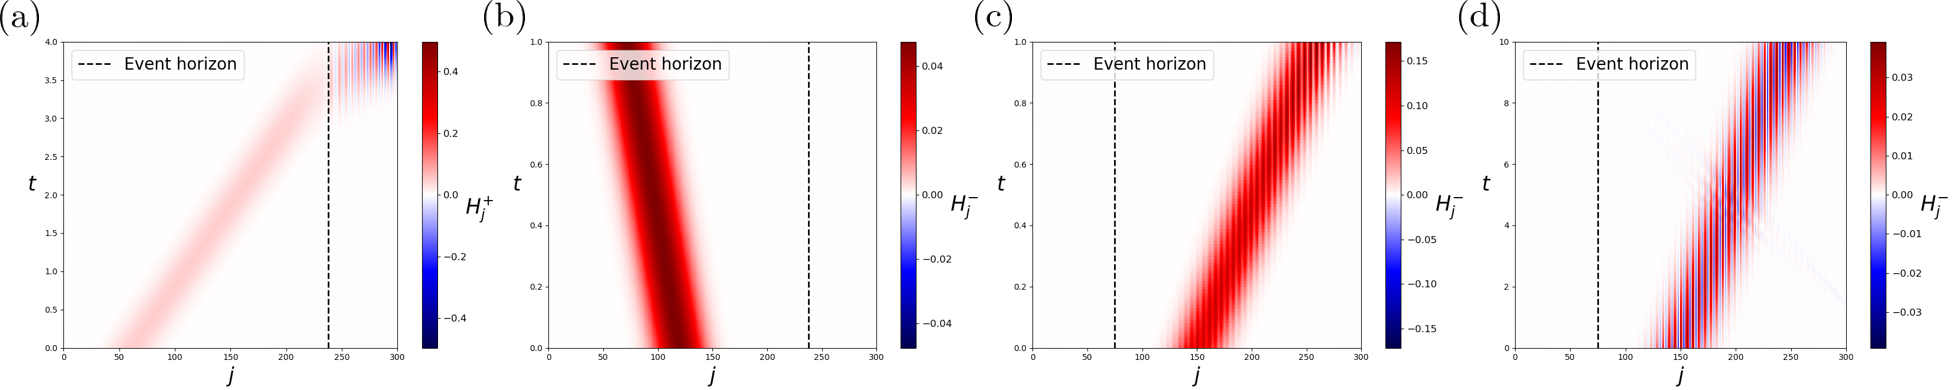
\includegraphics[width=\linewidth]{figure/p=1_BH.png}
\caption{Wave packet dynamics for the black hole profile with $p=1$. System parameters are the same as in Fig.~\ref{fig:bh_p0}: in (a,b), $x_0=2\ell/3$ and $j_h\approx213$; in (c,d), $x_0=\ell/3$ and $j_h\approx113$. (a) Packet initialized outside the horizon with ingoing group velocity ($j_0=30$, $\sigma=0.05L$). (b) Packet initialized outside the horizon with outgoing group velocity ($j_0=40$, $\sigma=0.05L$). (c) Packet initialized inside the horizon with a right-moving initial spinor ($j_0=180$, $\sigma=0.05L$). (d) Packet initialized inside the horizon with a left-moving initial spinor ($j_0=180$, $\sigma=0.05L$). Red dashed lines indicate the event horizon, and cyan curves indicate the corresponding null geodesics $dx/dt=\beta(x)\pm1$. Interior oscillations in (c,d) are more pronounced than in the $p=0$ case owing to the stronger excitation of doubler modes, as confirmed by the $k$-space analysis of Fig.~\ref{fig:doubler_fft}.}
\label{fig:bh_p1}
\end{figure*}
Next, we investigate the motion of the wave packet for the case $p=1$.
As in the case $p=0$, Figs.~\ref{fig:bh_p1}(a,b) show that wave packets initially placed outside the black hole follow the corresponding geodesic trajectories for both ingoing and outgoing motion.
Figs.~\ref{fig:bh_p1}(c,d) show that wave packets initially placed inside the black hole again propagate toward increasing $x$, as expected from the positive characteristic velocities inside the horizon.
Inside the black hole, the wave packet exhibits pronounced oscillatory behavior, whose origin can be traced to the doubler modes.
For the packet entering from the exterior [Fig.~\ref{fig:bh_p1}(a)], the oscillation develops after the packet reaches the interior.
This is caused by the excitation of doubler modes during time evolution.
Fig.~\ref{fig:doubler_fft}(a) shows the low-energy doubler modes that appear for $p=1$ inside the horizon, where $\beta>1$, while Fig.~\ref{fig:doubler_fft}(b) shows a secondary Fourier peak growing near the predicted wavenumber.
On the other hand, the oscillations in Figs.~\ref{fig:bh_p1}(c,d) are already present from the initial time.
Since these wave packets are initialized inside the black hole, they already have overlap with the doubler branch indicated in Fig.~\ref{fig:doubler_fft}(a).
Although the $p=0$ model also contains a doubler branch near $k=\pi$, the FFT analysis shows a larger doubler-mode peak for $p=1$ in the black hole interior, explaining the more pronounced oscillations in Figs.~\ref{fig:bh_p1}(c,d).
\begin{figure}[t]
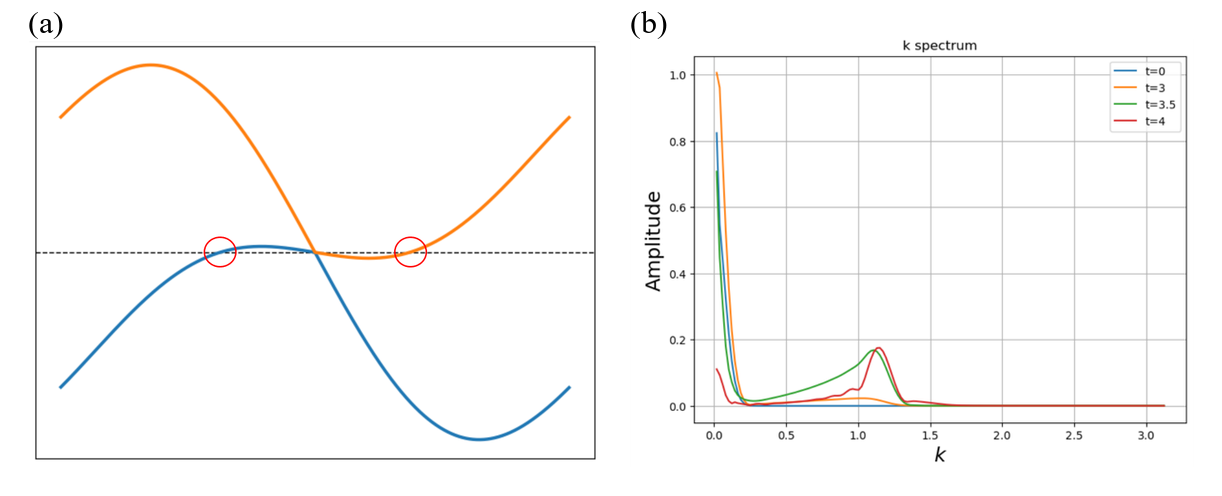
\includegraphics[width=\linewidth]{figure/doubler_fft.png}
\caption{Excitation of doubler modes in the oscillatory wave packet dynamics for $p=1$. (a) Dispersion relation at $\beta=1.2$, representative of the black hole interior. The circled low-energy crossings indicate doubler modes. (b) FFT spectrum of the wave packet inside the black hole at successive times $t=0,3,3.5,4$. The dominant peak near $k=0$ reflects the low-momentum quasiparticle, while the secondary peak is the doubler-mode peak and grows near the wavenumber predicted from (a). The spectrum confirms that the oscillatory behavior in Fig.~\ref{fig:bh_p1}(c,d) originates from the excitation of doubler modes.}
\label{fig:doubler_fft}
\end{figure}

We next extract the surface gravity of the effective horizon from the near-horizon wave packet dynamics.
For a left-moving wave packet localized in the exterior region near the event horizon, the linearized near-horizon null-geodesic equation gives the approximate growth of the standard deviation
\begin{align}
    \delta\sigma(t) \propto e^{\kappa t}-1,
    \label{eq:sigma_kappa}
\end{align}
where $\kappa=|\beta'(x_h)|$ is the surface gravity.
This approximate relation follows by linearizing the left-moving null trajectory $dx/dt=\beta(x)-1$ near the horizon, where $\beta(x_h)=1$, giving $d(x-x_h)/dt\simeq\kappa(x-x_h)$ and hence exponential stretching of the wave packet.
It implies that the surface gravity can be read off from the exponential growth rate of $\delta\sigma$ as long as the wave packet remains in the near-horizon regime.

For the surface-gravity extraction (Fig.~\ref{fig:sg}), we use $A=1$, $B=1$, $C=1$, $x_0=\pi$ (so $x_h=x_0$, $\kappa=|\beta'(x_h)|=1$, and $j_h=0.5L$), $j_0=245$, $\sigma=0.003L$, and fit the data over the time interval $t\in[0,1]$.
\begin{figure}[t]
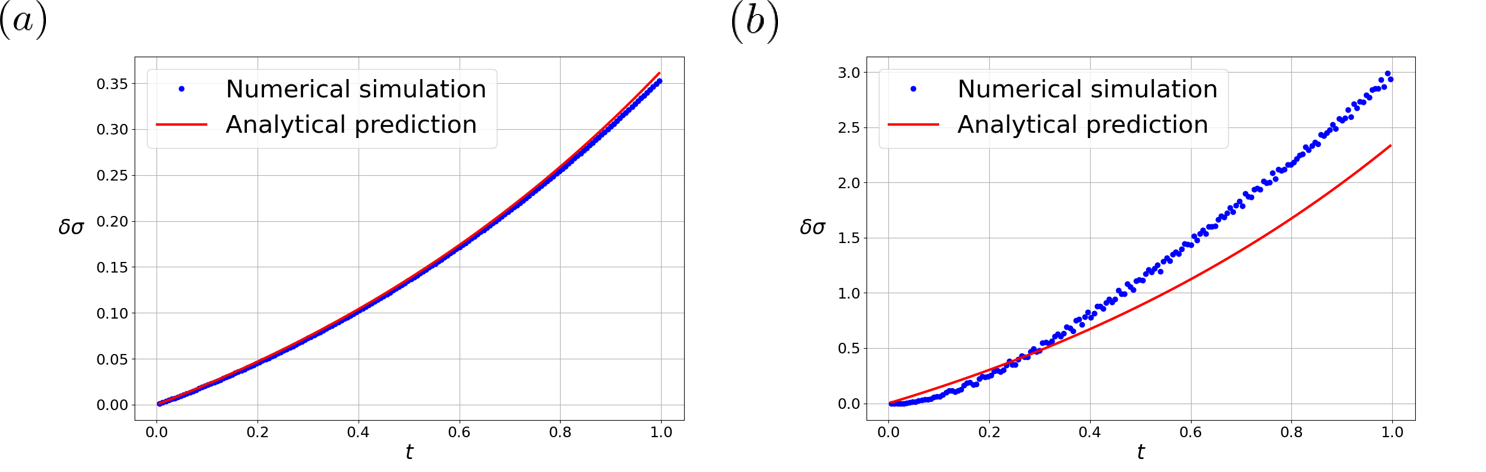
\includegraphics[width=\linewidth]{figure/sg.png}
\caption{Extraction of surface gravity from wave packet broadening ($L=300$, $A=B=C=1$, $x_0=\pi$, $\kappa=1$, $j_0=245$, $\sigma=0.003L$, with the fit performed over $t\in[0,1]$). Blue dots show the numerical simulation results, and red curves show the near-horizon approximation in Eq.~\eqref{eq:sigma_kappa}. (a) Result for $p=0$, with relative error $\approx2\%$. (b) Result for $p=1$, with relative error $\approx6\%$ due to simultaneous wave packet dispersion. The vertical axis $\delta\sigma\equiv\sigma(t)-\sigma(0)$ denotes the change in the wave-packet standard deviation.}
\label{fig:sg}
\end{figure}
Fig.~\ref{fig:sg} compares the numerical data with the analytical prediction.
As shown in Fig.~\ref{fig:sg}(a), for $p=0$, the extracted value agrees with the analytical value within a relative error of approximately 2\%.
The deviation from the analytical prediction increases with time, which can be attributed to the breakdown of the approximation in Eq.~\eqref{eq:sigma_kappa} as the wave packet moves away from the event horizon.

In contrast, for $p=1$, the discrepancy is larger than in the $p=0$ case.
The relative error with respect to the analytical value is about 6\%.
This discrepancy is likely due to deformation of the wave packet as it broadens, which causes deviations from the simple exponential behavior.

\subsection{White Hole}
In this section, we present the results of numerical simulations of particle dynamics in a white-hole spacetime. We consider the case in which a wave packet is incident from the exterior toward the interior of the white hole. We also discuss the finite-size effects that arise in this setup.
For the white-hole dynamics, we use $A=C=-0.6$, $B=3$, $x_0=7\pi/5$ (white-hole horizon at $j_h\approx0.743L$), with $j_0=0.2L$ and $\sigma=0.05L$.
\begin{figure}[t]
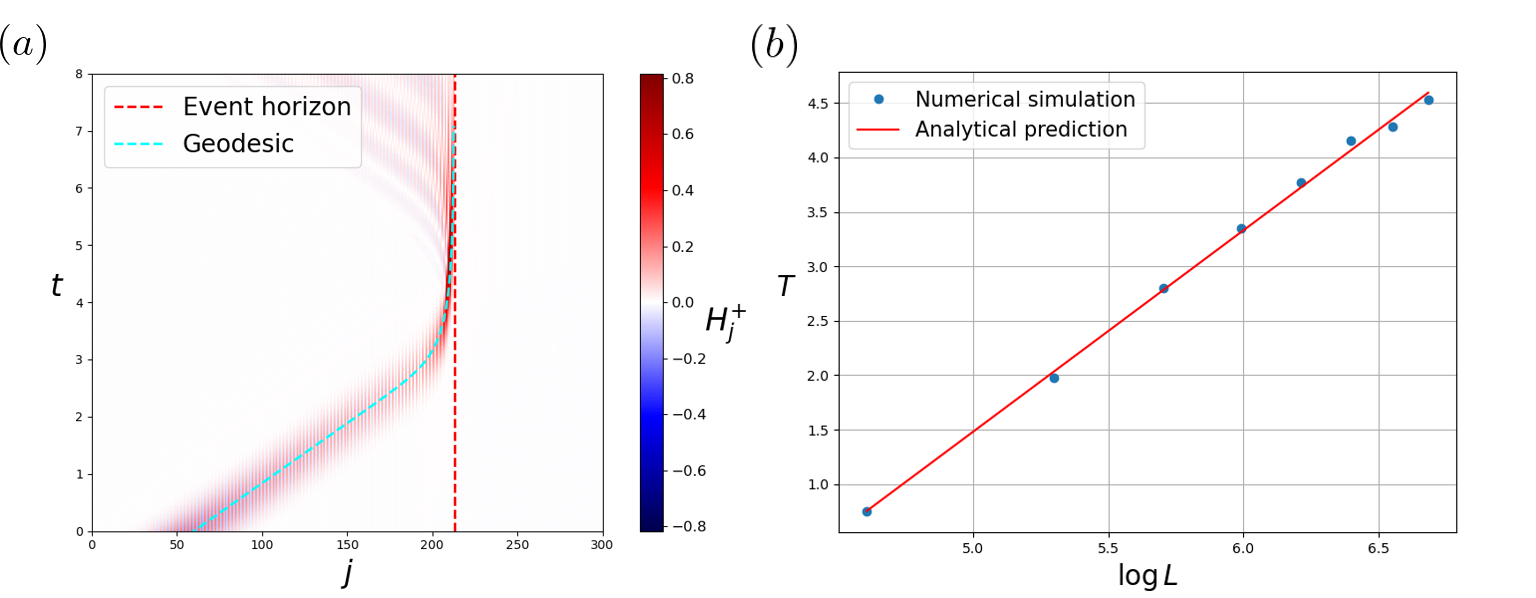
\includegraphics[width=\linewidth]{figure/WH_p=0.png}
\caption{Wave packet dynamics in the white-hole geometry for $p=0$. (a) Space-time diagram of $\mathcal{H}_j^+$ for $L=300$, $j_0=0.2L$, and $\sigma=0.05L$, with $\beta$ profile parameters $A=C=-0.6$, $B=3$, and $x_0=7\pi/5$ (white-hole horizon at $j_h\approx0.743L$). The wave packet is compressed toward the white-hole horizon (red dashed line) and eventually reflected due to finite lattice resolution. (b) Lattice stagnation time $T_{\mathrm{lat}}$ versus $\log L$ for various system sizes, using $A=C=-1$, $B=0.75$, $x_0=9\pi/5$, $j_0=0.2L$, and $\sigma=0.05L$. Blue dots show numerical simulation results, and the red line shows a linear fit, confirming the scaling of Eq.~\eqref{eq:T_logL}.}
\label{fig:wh_p0}
\end{figure}
For $p = 0$, as shown in Fig.~\ref{fig:wh_p0}, the wave packet is initially compressed at the white-hole horizon, yielding behavior consistent with the ideal analytical expectation. However, after a certain time, the wave packet collapses and is reflected. This behavior is attributed to a finite-size effect arising when the wave-packet standard deviation becomes smaller than the lattice spacing.
For the stagnation-time scaling in Fig.~\ref{fig:wh_p0}(b), we use a shallower profile, $A=C=-1$, $B=0.75$, and $x_0=9\pi/5$ ($x_h=x_0$ and $j_h=0.9L$), so that the linear near-horizon approximation remains valid over a wider spatial region.
Near the white-hole horizon, the same linearized null-geodesic argument gives an exponential compression of the wave-packet standard deviation, $\sigma(t)\propto\sigma_0 e^{-\kappa t}$.
In the lattice model, this continuum description breaks down once this standard deviation becomes comparable to the lattice spacing $\varepsilon=\ell/L$.
Defining the continuum estimate of the stagnation time $T_{\mathrm{cont}}$ by $\sigma(T_{\mathrm{cont}})\sim\varepsilon$, one obtains
\begin{align}
    T_{\mathrm{cont}} \propto \log L ,
    \label{eq:T_logL}
\end{align}
for fixed continuum size $\ell$ and fixed initial physical standard deviation $\sigma_0$.

We then test this logarithmic scaling by examining the dependence of the lattice stagnation time $T_{\mathrm{lat}}$ on the system size $L$.
To define $T_{\mathrm{lat}}$ in the numerical data, we first identify the time $t_{\mathrm{in}}$ at which the second derivative of $\beta$ evaluated at the wave-packet mean position falls below $0.1$.
We then identify the time $t_{\mathrm{min}}$ at which the wave-packet standard deviation reaches its minimum.
The lattice stagnation time is defined as $T_{\mathrm{lat}} = t_{\mathrm{min}} - t_{\mathrm{in}}$.
The results shown in Fig.~\ref{fig:wh_p0} confirm that $T_{\mathrm{lat}}$ follows the scaling predicted for $T_{\mathrm{cont}}$.
Therefore, we conclude that the reflection of the wave packet is caused by a finite-size effect associated with its standard deviation becoming smaller than the lattice spacing.

\begin{figure}[t]
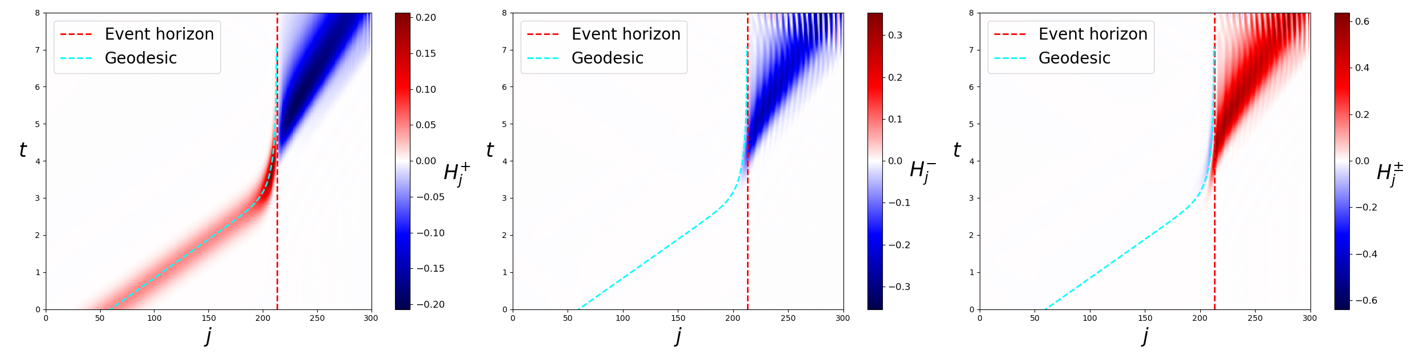
\includegraphics[width=\linewidth]{figure/WH_p=1.png}
\caption{White-hole dynamics for $p=1$ ($L=300$, $j_0=0.2L$, $\sigma=0.05L$, with the same $\beta$ profile as Fig.~\ref{fig:wh_p0}(a), $A=C=-0.6$, $B=3$, $x_0=7\pi/5$, and $j_h\approx0.743L$). (a) Space-time diagram of $\mathcal{H}_j^+$. (b) Space-time diagram of $\mathcal{H}_j^-$. (c) Space-time diagram of $\mathcal{H}_j^\pm$. Unlike the $p=0$ case, the coupling between the right- and left-moving components allows partial transmission across the white-hole horizon (red dashed line).}
\label{fig:wh_p1}
\end{figure}
For $p=1$, the wave packet dynamics differs from the $p=0$ case.
As shown in Fig.~\ref{fig:wh_p1}, part of the wave packet crosses the white-hole horizon instead of being simply reflected.
This behavior is absent for $p=0$ and suggests a role of the coupling between the right- and left-moving modes.

\section{CONCLUSIONS}
In this work, we have investigated particle dynamics in a one-dimensional lattice fermion model designed to simulate black hole and white-hole spacetimes, focusing on the correspondence between lattice wave packet trajectories and geodesics of the effective curved metric.

For the black hole geometry, Gaussian wave packets initialized both outside and inside the event horizon closely follow the corresponding geodesics for both $p=0$ and $p=1$ parameter choices. The oscillatory behavior observed inside the black hole arises from doubler modes, with the $p=1$ case exhibiting more pronounced oscillations owing to stronger overlap with, and excitation of, these modes. We also extracted the surface gravity from the exponential growth of the wave-packet standard deviation in the near-horizon regime, finding agreement within a relative error of $\sim 2\%$ for $p=0$ and a larger discrepancy of $\sim 6\%$ for $p=1$, with the latter attributed to deformation of the wave packet during broadening.

For the white-hole geometry, the wave packet is compressed toward the white-hole horizon in a manner consistent with the continuum expectation, but eventually collapses and reflects due to a finite-size effect. The lattice stagnation time follows the logarithmic system-size scaling $T_{\mathrm{lat}}\propto\log L$, as confirmed numerically. For $p=1$, partial transmission across the white-hole horizon is observed, suggesting an important role of the coupling between left- and right-moving modes.

These results demonstrate that the one-dimensional lattice fermion model provides a practical framework for assessing curved-spacetime particle dynamics in lattice fermion simulators. Future directions include extending the model to time-dependent backgrounds to study particle-creation phenomena such as Hawking radiation and cosmological particle production, as well as implementing the lattice Hamiltonian on near-term quantum hardware to experimentally probe these phenomena.

\bibliography{books}

\end{document}
